\newpage
\section{Umsetzung}
\label{Umsetzung}
Nachdem die theoretischen Grundlagen im letzten Kapitel vorgestellt wurden, wird in diesem Kapitel die Umsetzung beschrieben. Dieses Kapitel wird nach einem geordneten Vorgehen strukturiert. Zuerst werden verfügbare Daten vorgestellt, analysiert und sortiert. In diesem Schritt wird entschieden, welche Daten die Zielvariable Nachfrage beeinflussen und somit mit in das Modell eingegeben werden. Die deskriptive Analyse unterstützt dabei die Visualisierung der Daten und verleiht mehr Verständnis für den zeitlichen Einsatz und die Verteilung der Kosten innerhalb der Medienkanäle. Darauffolgend werden die Daten in das \ac{OLS}-Modell eingesetzt. Die Ergebnisse des Modells werden analysiert.

\subsection{Einsatz der deskriptiven Analyse}
\label{EinsatzDerDeskriptivenAnalyse}
Wie im Kapitel \nameref{deskriptiveanalyse} beschrieben, fasst die deskriptive Analyse historische Daten zusammen und zeigt wichtige Muster und Trends auf. Sie bildet die Grundlage für weiterführende Analysen und datengestützte Entscheidungen. Um auf den Einsatz des \ac{OLS}-Modells vorzubereiten, werden die Daten vom \ac{MMM} deskriptiv analysiert. \\\\
Für das \ac{MMM}-Modell (s. \autoref{fig:mmmbonprix}) stehen Daten vom 01.01.2022 bis 31.12.2024 zur Verfügung. Diese Daten umfassen die Marketing-Ausgaben, wie Katalogausgaben, Online-Marketingausgaben und Mediaausgaben. Für Mediakanäle sind spezifisch auch die Kosten der Unterkanäle dabei. 
Unter diesen Daten fallen auch Kosten für (adressierbares) TV, Podcasts, \ac{dooh}+\ac{ooh}, Radio, YouTube, soziale Medien, Online-Videos und Display-Medien. Für die internen Faktoren sind Kosten von E-Mail, Push-Nachrichten und Verkaufsförderungen wie Versandkostenbefreiung und Rabatt verfügbar. Für die externen Faktoren ist ein Saisonalitätswert von einem Facebook-Saisonmodell vorhanden. Um die Wettbewerber im Modell zu berücksichtigen, sind auch Marketingausgaben von C\&A, H\&M, About You und Zalando verfügbar. Zum Schluss ermöglichen Nachfrage und Datum, den Verlauf sowie die Auswirkungen aller Faktoren auf Tagesbasis darzustellen. \\\\
Da es auf der Media-Ebene modelliert wird, werden nicht alle Daten von dem \ac{MMM} benötigt. Für den Anfang werden nur für Media relevante Daten für das Modell entnommen. Die Daten werden von der Google BigQuery Cloud in die Google Jupyter-Notebook-Instanz geladen, um dort mit Python modelliert zu werden. Die Daten bilden eine Tabelle, in der jede Zeile nach Datum sortiert ist und einen Tag mit den Informationen aller Variablen darstellt. \\\\
Zuerst wird die Qualität der Daten für das \ac{MMM} überprüft. Wie im \autoref{methodederkleinstenquadrate} beschrieben, führen Redundanzen zu einem falschen Ergebnis im Modell. Deshalb soll es überprüft werden, ob es allgemein Redundanzen in den Zeilen gibt. Auch ohne \(y_i\) kann der Koeffizient $\beta$ nicht geschätzt werden. In dem Media-Modell ist die Nachfrage der Zielwert \(y_i\), da es gerechnet werden soll, wie viel ein Euro als Ausgabe in einem Media-Kanal in der Nachfrage bringt. Die Nachfrage darf deswegen nicht Null sein. Daher wird im ersten Schritt überprüft, ob allgemein Redundanzen vorliegen und ob in der Spalte \anf{demand} Nullwerte vorhanden sind.\\\\
So wurde der Code \verb|df_raw[df_raw['demand'].isnull()]| ausgeführt, um Zeilen mit einem leeren Nachfrage-Wert abzufragen. Dabei wurde eine Zeile mit einem leeren Nachfrage-Wert am 29.06.2024 identifiziert. Um den Null-Wert zu korrigieren, wurde der Durchschnitt der Nachfragen am 28.06.2024 und am 30.06.2024 für das Datum 29.06.2024 berechnet und eingesetzt.  
\begin{lstlisting}[language=Python, linewidth=\textwidth]
mask = (df_raw['date'] == '2024-06-29')
avg_demand = df_raw.loc[df_raw['date'].isin(['2024-06-28', '2024-06-30']), 'demand'].mean()
df_raw.loc[mask, 'demand'] = avg_demand
\end{lstlisting}
Nach der Datenverarbeitung wurde ein Überblick über den Datenverlauf geschaffen, um die erste Forschungsfrage in \nameref{ZielsetzungDerArbeit}
zu beantworten. Es wurde untersucht, wie sich die Mediaausgaben verhalten und welche möglichen Auswirkungen sie auf die Nachfrage haben. Mithilfe des Codes im \nameref{Anhang1:ZeitlicherVerlaufMitPywidgets} wird ein Liniendiagramm erstellt, bei dem die x-Achse die Zeit auf Tagesbasis darstellt. Die linke y-Achse zeigt die prozentualen Werte für die Ausgaben der Media-Kanäle, während die rechte y-Achse die prozentualen Werte für die Nachfrage darstellt. Um die Visualisierung flexibel zu gestalten, wird mithilfe von \verb|ipywidgets| eine interaktive Datendarstellung mit Auswahllisten erstellt. Diese Auswahllisten ermöglichen es, zwischen verschiedenen Media-Kanälen zu wechseln und ein flexibles Startdatum zwischen dem 01.01.2022 und dem 01.01.2025 für die x-Achse im Diagramm auszuwählen. Die prozentualen Werte der y-Achsen werden berechnet, indem die Tagesausgaben durch die Gesamtausgaben dividiert werden. Die Berechnung der prozentualen Werte ermöglicht einen besseren Vergleich zwischen den beiden Werten und vermeidet eine Darstellung mit absoluten Zahlen. Diese Ausgaben werden nach der Auswahl eines Datums neu berechnet, um eine zeitgemäße Darstellung zu gewährleisten. \\\\
Das Kapitel \nameref{MediaKanäleInDerPraxis} beschreibt, dass Generali eine gute Erfahrung mit YouTube als Media-Kanal hat. Auch die Metaanalyse von Nielsen besagt, dass YouTube beim \ac{ROI} das TV übertrifft. Also wird der YouTube-Verlauf mit dem Verlauf der Nachfrage zuerst verglichen:\\\\
\begin{figure}[ht]
    \centering
    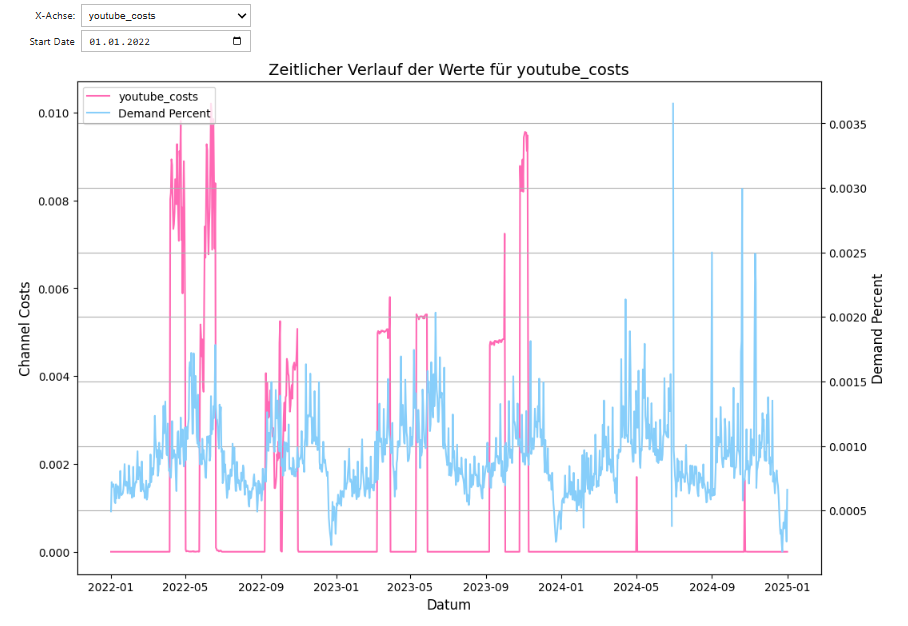
\includegraphics[width=0.98\linewidth]{images/youtubeLineChart.png}
    \caption{Liniendiagramm: Ein Vergleich von YouTube-Ausgaben und Nachfrage, eigene Darstellung}
    \label{fig:youtubelinechart-label}
\end{figure}
\noindent
Aus dem Liniendiagramm in \autoref{fig:youtubelinechart-label} geht hervor, dass die YouTube-Ausgaben sporadisch auftreten. Wie im \autoref{MediaKanäleBeiBonprix} beschrieben, entstehen Ausgaben für diesen Media-Kanal in einem begrenzten Zeitraum, etwa für einen Monat. Auch hier ist es zu erkennen, dass für den Kanal YouTube zweimal Kosten anfallen, mit einem kurzen zeitlichen Abstand. Die YouTube-Ausgaben treten meist um Mai und kurz nach September auf. Dies ist auch der Zeitraum, in dem die Nachfrage etwas höher ist. \\\\
Mit bloßem Auge ist nicht erkennbar, ob ein Zusammenhang zwischen den Mediaausgaben und der Nachfrage besteht. Allerdings ähnelt der Verlauf der Online-Marketingausgaben dem Verlauf der Nachfrage. Im Liniendiagramm in \autoref{fig:omaverlauf} ist zu erkennen, dass der Verlauf von Online-Marketing und Nachfrage nahezu übereinstimmt. Das weist darauf hin, dass das Online-Marketing möglicherweise einen großen Einfluss auf die Nachfrage hat und im Modell zu berücksichtigen ist.
\begin{figure}[H]
    \centering
    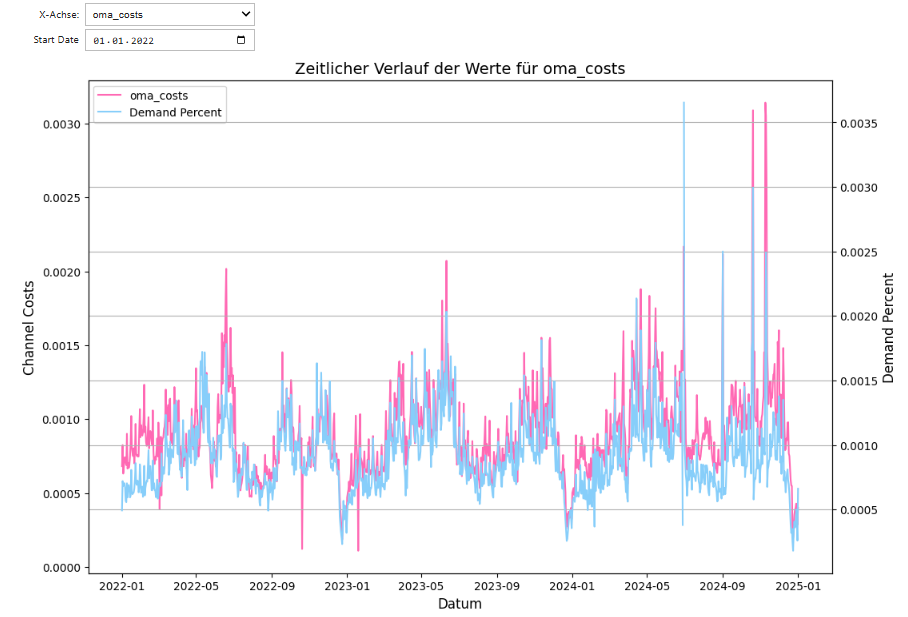
\includegraphics[width=1\linewidth]{images/omacosts.png}
    \caption{Verlauf von Ausgaben des Online-Marketings und Nachfrage ab 01.01.2022, eigene Darstellung}
    \label{fig:omaverlauf}
\end{figure}
\noindent
Neben dem Online-Marketing hat auch die Verkaufsförderung einen möglichen Einfluss auf die Nachfrage. In \autoref{fig:verlaufvonverkaufsförderung} ist zu erkennen, dass zwischen Juli 2024 und Dezember 2024 vier hohe Spitzen der Nachfrage und Verkaufsförderungskosten parallel entstanden sind. 
\begin{figure}[H]
    \centering
    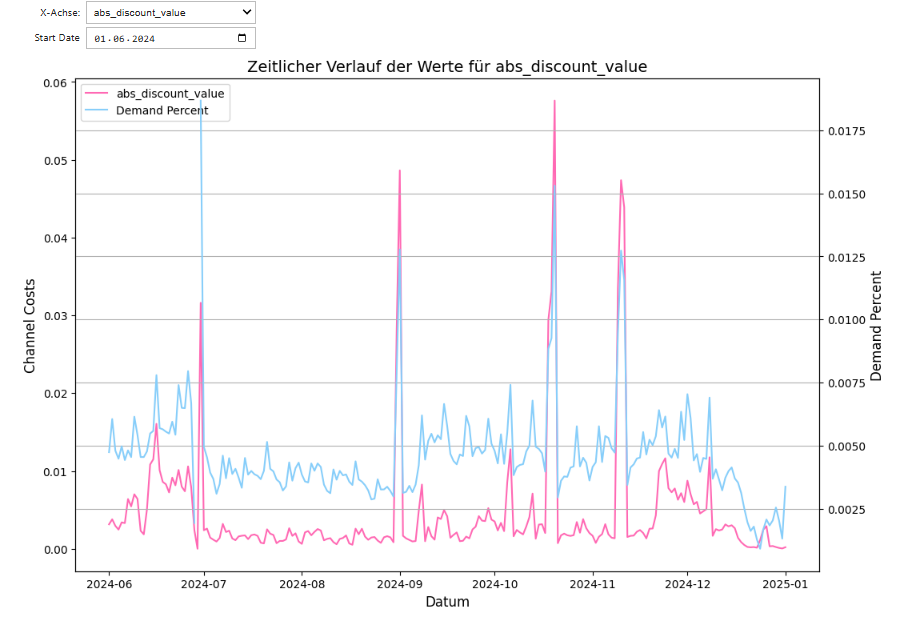
\includegraphics[width=1\linewidth]{images/vf_sum.png}
    \caption{Verlauf von Verkaufsförderung und Nachfrage ab 01.06.2024, eigene Darstellung}
    \label{fig:verlaufvonverkaufsförderung}
\end{figure}
\noindent
Es wird erwartet, dass Einflussfaktoren wie Online-Marketing und Verkaufsförderung einen sofortigen Einfluss auf die Nachfrage haben. Eine Erhöhung der Ausgaben für solche Faktoren führt zu einem sofortigen Anstieg der Nachfrage. Im Vergleich dazu haben Medienkanäle wie YouTube keinen direkt erkennbaren Effekt auf die Nachfrage. Es wird angenommen, dass der Effekt von Media-Kanäle milder und nachhaltiger auf das Konsumverhalten ist. Um den Nachfrageeffekt von Media-Kanäle zu quantifizieren, werden später die \ac{OLS}-Funktion und die Huber-Regression eingesetzt und der \ac{ROAS} berechnet.
\begin{figure}[H]
    \centering
    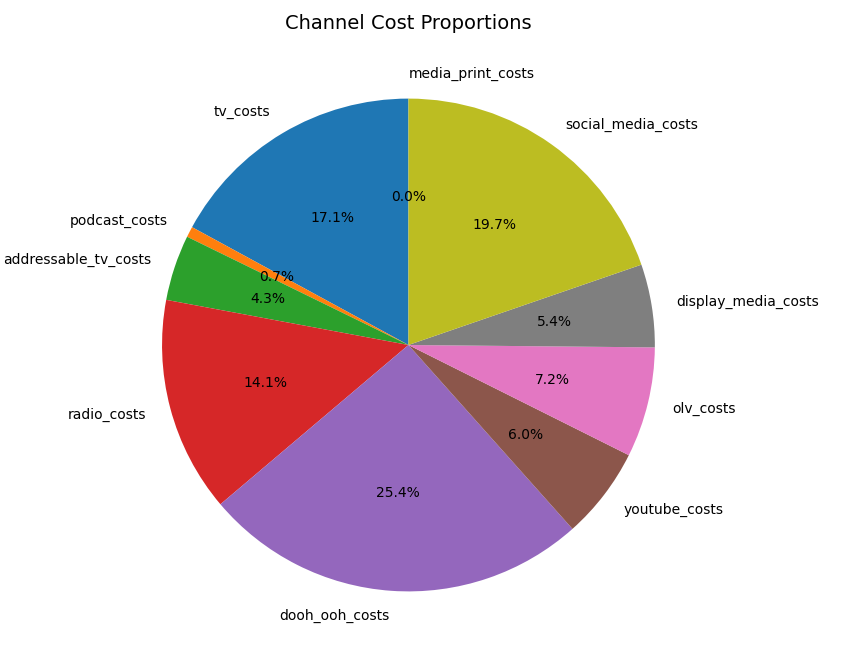
\includegraphics[width=0.8\linewidth]{images/mediapie.png}
    \caption{Kostenanteil der Marketingkanäle im Zeitraum vom 1.1.2022 bis zum 31.12.2024 bei bonprix, eigene Darstellung.}
    \label{fig:mediapie}
\end{figure}
\noindent
Um die Verteilung der Ausgaben für Media-Kanäle besser zu verstehen, werden die Ausgabenanteile der Media-Kanäle in einem Kreisdiagramm visualisiert. Der Code im \nameref{Anhang2KreisdiagrammAufteilungDerMediaausgaben} ermöglicht ebenfalls die Interaktion mit dem Startdatum und erstellt das Kreisdiagramm in \autoref{fig:mediapie} mit einem Startdatum von 01.01.2022.\\\\
% ROI
In diesem Kreisdiagramm in \autoref{fig:mediapie} ist es zu erkennen, dass die YouTube-Ausgaben einen relativ kleinen Anteil von 6\% betragen. Das entspricht etwas mehr als einem Drittel der TV-Ausgaben, die 17,1 \% betragen. Wenn \nameref{MediaKanäleInDerPraxis} zutrifft, dass YouTube mehr \ac{ROI} als TV erbringt und wenn die Trainingsdaten vollständig sind, wird erwartet, dass YouTube einen höheren \ac{ROAS} als TV aufweist. Es wird erwartet, dass in der optimalen Aufteilung YouTube einen höheren Anteil als in der Gegenwart aufweist. Die höchsten Kosten entfallen auf die Kombination von \ac{dooh} und \ac{ooh}, die einen Anteil von 25,4 \% aufweist.
\newpage
\subsection{Prüfung und Umgang mit Multikollinearität}
\label{PrüfungUndUmgangMitMultikollinearität}
Wie im \autoref{einschränkungenderregression} beschrieben, muss die Kollinearität zwischen den Prädiktoren behoben werden. Als Erstes wird die Korrelationsmatrix der Prädiktoren, alle Unterkanäle in Media, untersucht. Mithilfe der Methode \verb|.corr()| wird die Korrelation zwischen den Prädiktoren berechnet. Anschließend wird die Korrelation mit der Funktion \verb|.heatmap| aus der Bibliothek \verb|seaborn| farblich visualisiert.
\begin{figure}[H]
    \centering
    \begin{lstlisting}[language=Python, linewidth=\textwidth]
df_corr_media=dfcmedia.corr() 
plt.figure(figsize=(15, 12))
sns.heatmap(df_corr_media, annot=True, cmap='coolwarm', fmt=".2f")
plt.title("Korrelationsmatrix")
plt.show()
\end{lstlisting}
    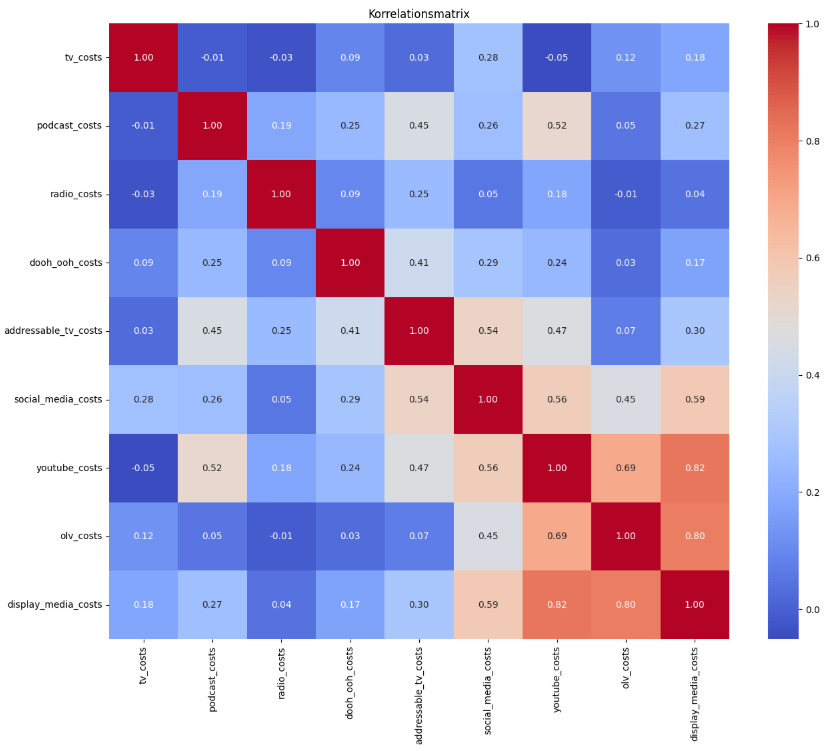
\includegraphics[width=0.9\linewidth]{images/korrelationsmatrix.png}
    \caption{Korrelationsmatrix der Prädiktoren, eigene Darstellung}
    \label{fig:korrelationsmatrix}
\end{figure}
Wie im \autoref{einschränkungenderregression} beschrieben, weist ein großer absoluter Wert in der Korrelationsmatrix auf eine hohe Korrelation hin. Das bedeutet, dass sowohl Werte nahe -1 als auch nahe 1 eine hohe Korrelation beschreiben. Die negative Korrelation ist unproblematisch, da der Betrag der negativen Werte alle gleich oder unter 0,05 bleibt. Hingegen ist die positive Korrelation problematisch. Paare wie YouTube mit Display Media, \ac{olv} mit Display Media, YouTube mit \ac{olv}, YouTube mit Social Media, Social Media mit Display Media haben alle einen Wert von mindestens 0,56. \\\\
Es wird mit einer Untersuchung von \ac{VIF} fortgesetzt. Zuerst werden numerische Werte herausgefiltert. Danach werden Werte ohne Veränderung, also Standardabweichung gleich 0, mit \verb|.std() > 0| entfernt. Zum Schluss wird mithilfe der Methode \verb|variance_inflation_factor()| der \ac{VIF} ausgerechnet. 
\begin{lstlisting}[language=Python, linewidth=\textwidth][H]
X = X.select_dtypes(include=[np.number]) 
X = X.loc[:, X.std() > 0]
vif = pd.DataFrame()
vif["Variable"] = X.columns
vif["VIF"] = [variance_inflation_factor(X.values, i) for i in range(X.shape[1])]
print(vif)
\end{lstlisting}
\begin{table}[h]
    \centering
    \begin{tabular}{@{}ll@{}}
        \toprule
        Variable               & VIF       \\ \midrule
        tv\_costs              & 1.376725  \\
        podcast\_costs         & 1.946688  \\
        addressable\_tv\_costs & 2.257337  \\
        radio\_costs           & 1.143652  \\
        dooh\_ooh\_costs       & 1.321926  \\
        youtube\_costs         & 7.717482  \\
        olv\_costs             & 4.336781  \\
        display\_media\_costs  & 6.224349  \\
        social\_media\_costs   & 2.658416  \\ \bottomrule
    \end{tabular}
    \label{tab:viftabelle}
    \caption{Variance Inflation Factor (VIF) for Variables, eigene Darstellung}
\end{table}
In der \hyperref[tab:viftabelle]{Tabelle VIF} wird erkannt, dass YouTube und Display Media jeweils einen \ac{VIF}-Wert über 5 besitzen. Nach \autoref{einschränkungenderregression} werden sie als problematisch eingestuft. Basierend auf den Erfahrungen in der Abteilung wird ein \ac{VIF}-Wert ab 2 als problematisch angesehen. \ac{olv}, Social Media und eventuell adressierbarer TV werden daher als problematisch betrachtet. Dies bestätigt auch die hohen Korrelationswerte in der \autoref{fig:korrelationsmatrix}. Nach dem Austausch mit der Media-Abteilung wird bestätigt, dass Display Media, YouTube, \ac{olv} und Social Media oft zusammen aktiviert werden. In der Analyse werden diese Kanäle deshalb als Variable \verb|video_costs| zusammengefasst: 
\begin{lstlisting}
df["video_costs"] = df["youtube_costs"] + df["olv_costs"] + 
                df["display_media_costs"] + df["social_media_costs"]
\end{lstlisting}
Nach der Verarbeitung von den Prädiktoren wird die hohe Korrelation in der Korrelationsmatrix in \autoref{fig:korrelationsmatrix-danach} beseitigt.
\begin{figure}
    \centering
    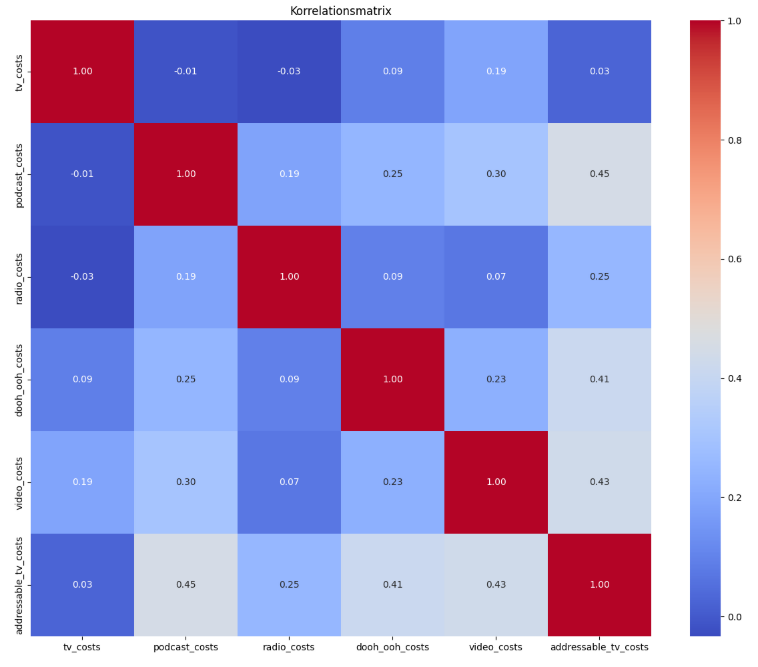
\includegraphics[width=0.75\linewidth]{images/korrelationafter.png}
    \caption{Korrelationsmatrix nach der Behebung von hoher Korrelation, eigene Darstellung}
    \label{fig:korrelationsmatrix-danach}
\end{figure}
Die \ac{VIF}-Werte dazu in \autoref{tab:small_vif} signalisieren auch einen sicheren Umgang mit der Kollinearität. 
\begin{table}[H]
    \centering
    \begin{tabular}{|l|r|}
        \hline
        \textbf{Feature} & \textbf{VIF} \\ 
        \hline
        tv\_costs            & 1.073154 \\
        podcast\_costs       & 1.333356 \\
        addressable\_tv\_costs & 1.792658 \\
        radio\_costs         & 1.141264 \\
        dooh\_ooh\_costs     & 1.341440 \\
        video\_costs         & 1.774887 \\
        \hline
    \end{tabular}
    \caption{VIF-Werte nach der Behebung der Kollinearität, eigene Darstellung}
    \label{tab:small_vif}
\end{table}
\subsection{Einsatz des Marketing-Mix-Modells}
\label{EinsatzDesMarketing-Mix-Modells}
Nachdem die \ac{VIF}-Werte verbessert worden sind, werden die Prädiktoren in das Modell eingesetzt. \\\\
Es gibt bereits eine interne \ac{MMM}-Bibliothek, die Marketing-Daten verarbeitet und transformiert, beispielsweise die Werbewirkung (Adstock), die im \autoref{Marketing-Mix-ModellBeiBonprix} beschrieben ist. Dabei wird angestrebt, den \ac{ROAS} für verschiedene Kanäle wie Media, \ac{OMA} und Katalog zu berechnen. Optional kann auch die Wavelet-Funktion aktiviert werden, die die Nachfragefunktion glättet. Dadurch wird erhofft, drastische Schwankungen in der Nachfrage zu entfernen. Drastische Schwankungen werden, wie im \autoref{deskriptiveanalyse} beschrieben, durch Aktionen wie Rabatte oder Online-Marketing verursacht. Außerdem haben Media-Kanäle ein Markenziel (siehe \nameref{MediaKanäleBeiBonprix}) und haben keinen sofortigen Einfluss auf die Nachfrage (siehe \nameref{deskriptiveanalyse}). Der Einsatz der Wavelet-Funktion zielt darauf ab, die grundlegende Kurve in der Nachfrage zu berechnen.  
\begin{lstlisting}[language=Python, linewidth=\textwidth]
model_specification = {'client_id': 2, 'regression': 'huber', 
    'levels_diff': 'levels', 'competitors': 'yes', 
    'interaction_effect': 'no', 
    'channels': ['oma_costs', 'media_costs', 'catalog_costs'],
    'target': 'demand', 'M_a': 21, 'start_date': '2020-01-01', 
    'end_date': '2025-01-01', 'trend': 'yes', 'wavelets': 'yes', 
    'wavelets_target': 'demand', 'wavelets_channel': 'media_costs'}
df_wlt_decomp = wavelet_trans(data_raw = df_raw, 
trans_target = model_specification['target'])
\end{lstlisting}
Die Wavelet-Funktion wird verwendet, um die Nachfrage über verschiedene Zeitspannen hinweg zu glätten. Im Modell werden Zeitspannen von jeweils 1, 2, 4, 8, 16, 32 und 64 Tagen verwendet. In der \autoref{fig:wavelet} wird die geglättete Nachfrage visualisiert. Die Funktion in Magenta ist die Nachfrage, geglättet über 8 Tage. Hierbei ist zu erkennen, dass die Funktion umso glatter wird, je mehr Tage geglättet werden. Die blaue Funktion auf der rechten Seite repräsentiert die Glättung über die höchste Tagesanzahl. Die drastischen Schwankungen auf Tagesbasis verschwinden. \\\\
In \autoref{lst:stargazer} werden Modellergebnisse ausgedruckt. Der Code wendet \ac{OLS} an und listet Modellergebnisse in einer Tabelle auf. In \verb|cost_columns| werden Kanalnamen gespeichert und durch \verb|join()| werden die Daten der Kanäle dementsprechend im Modell berücksichtigt. 
\begin{lstlisting}[language=Python, linewidth=\textwidth]
demand_days = [1, 2, 4, 8, 16, 32, 64]
regressions = []
for days in demand_days:
    reg = sm.OLS.from_formula(f"demand_{days}d ~ " + " + ".join(cost_columns), df_wlt_decomp).fit()
    regressions.append(reg)
results_table = Stargazer(regressions)
results_table.custom_columns(['Daily', '2Days', '4Days', '8Days', '16Days', '32Days', '64Days'], [1, 1, 1, 1, 1, 1, 1])
results_table.show_model_numbers(False)
results_table
\end{lstlisting}
\label{lst:stargazer}
\begin{figure}[H]
    \centering
    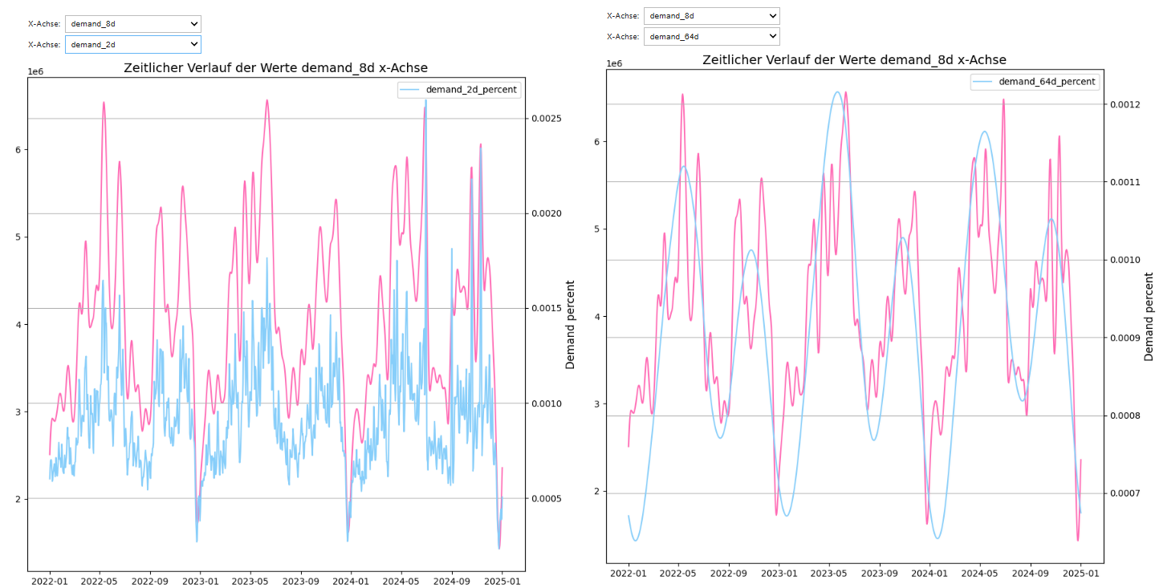
\includegraphics[width=1\linewidth]{images/wavelet.png}
    \caption{Nachfrage-Funktion, geglättet durch die Wavelet-Funktion}
    \label{fig:wavelet}
\end{figure}
\begin{figure}
    \centering
    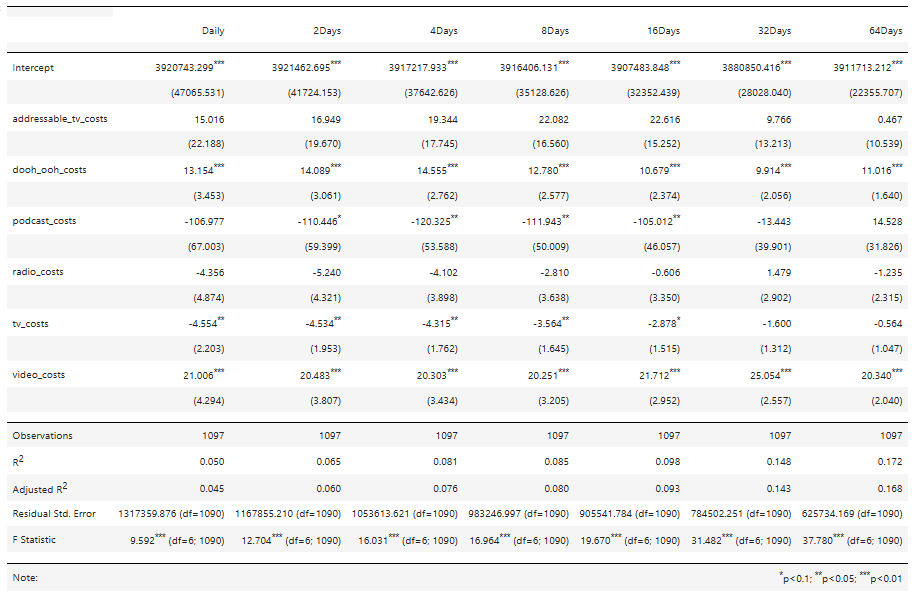
\includegraphics[width=1\linewidth]{images/ols1.png}
    \caption{\ac{OLS} Modellergebnis mit Media-Kanäle}
    \label{fig:ols1}
\end{figure}
Die Modellergebnisse in \autoref{fig:ols1} zeigen unrealistische Werte. Die Zahlen in der Tabelle sollen \ac{ROAS}-Werte darstellen. Laut \autoref{AnpassungsgüteUndDieVarianzanalyse} ist 5 \% ein Richtwert für das Signifikanzniveau. Daher sind Werte mit mindestens zwei Sternchen (\(**p < 0,05\)) signifikant. Die \verb|video_costs| führen laut Modellergebnissen zu einem \ac{ROAS} von 21 Euro pro investiertem Euro auf Tagesbasis, während \ac{dooh}/\ac{ooh} einen \ac{ROAS} von 13 Euro erzielen. Die drei Sternchen deuten zudem auf eine hohe Signifikanz hin und das ist unmöglich. Das Bestimmtheitsmaß mit 0,05 auf Tagesbasis ist sehr niedrig. In \autoref{AnpassungsgüteUndDieVarianzanalyse} wird beschrieben, dass ein Bestimmtheitsmaß nahe 0 auf eine schlechte Anpassungsgüte des Modells hinweist. Das bedeutet für das Modell, dass nur 5 \% der Gesamtvariation in der Nachfrage durch die Variation der Prädiktoren erklärt werden. Eine mögliche Ursache für das schlechte Ergebnis könnte das Fehlen wichtiger Prädiktoren sein. Die Nachfrageeffekte anderer Einflussfaktoren werden nicht berücksichtigt, und das Modell ordnet den Effekt den Media-Kanälen zu.\\\\
Das \ac{MMM} bei bonprix hat wie im \autoref{Marketing-Mix-ModellBeiBonprix} beschrieben einige große Einflussfaktoren. Die Konkurrenten, Saisonalität,  Mailversand, Verkaufsförderungen und andere Marketingkanäle wie Katalog und \ac{OMA}. Um wichtige Einflussfaktoren im Modell aufzunehmen, werden diese Prädiktoren in das Modell eingeführt. Da die Einheit des Mailversands in den Daten nicht in Euro, sondern in der Anzahl der Mails angegeben ist, werden diese zunächst nicht berücksichtigt. \\\\
Die Saisonalität von Meta \verb|pred_prophet|, Online-Marketing-Ausgaben \verb|oma_costs|, Trend \verb|trend|, Katalogausgaben \verb|catalog_costs_total|, Rabatt in Euro \verb|abs_discount_value|, Versandkostenbefreiung in Euro \verb|sum_vkb| sowie die Mediaausgaben von vier Konkurrenten werden entnommen und untersucht. Der Trend wird durch aufzählende Zahlen ab 1 definiert, wie im \nameref{Marketing-Mix-ModellBeiBonprix} bei \ac{MMM} beschrieben. Zuerst wird die Kollinearität aller Prädiktoren untersucht. Allerdings führt die Kombination der Prädiktoren zu hohen \ac{VIF}-Werten. \verb|oma_costs| weist einen \ac{VIF}-Wert von 29,8 auf, während \verb|pred_prophet| einen Wert von 18,25 aufweist. Beide Werte liegen über 10, was in der linearen Regression vermieden werden sollte.
\noindent
\begin{table}[H]
    \centering
    \begin{tabular}{@{}p{0.45\textwidth}@{\hskip 0.05\textwidth}p{0.45\textwidth}@{}}
        \begin{minipage}{0.45\textwidth}
            \centering
            \textbf{Tabelle mit trend und pred\_prophet} \\
            \begin{tabular}{|l|r|}
                \hline
                \textbf{Feature} & \textbf{VIF} \\ 
                \hline
                tv\_costs & 1.107315 \\
                podcast\_costs & 1.449923 \\
                addressable\_tv\_costs & 1.848572 \\
                radio\_costs & 1.192543 \\
                dooh\_ooh\_costs & 1.369786 \\
                video\_costs & 1.876529 \\
                oma\_costs & 29.821870 \\
                pred\_prophet & 18.257818 \\
                trend & 4.455062 \\
                catalog\_costs\_total & 1.064823 \\
                abs\_discount\_value & 3.273036 \\
                sum\_vkb & 2.472620 \\
                c\_and\_a\_costs & 1.865910 \\
                h\_and\_m\_costs & 1.603432 \\
                aboutyou\_costs & 1.602379 \\
                zalando\_costs & 1.949403 \\
                \hline
            \end{tabular}
        \end{minipage}%
        &
        \begin{minipage}{0.45\textwidth}
            \centering
            \textbf{Tabelle ohne trend und pred\_prophet} \\
            \begin{tabular}{|l|r|}
                \hline
                \textbf{Feature} & \textbf{VIF} \\ 
                \hline
            tv\_costs          & 1.091880 \\
            podcast\_costs     & 1.390602 \\
            addressable\_tv\_costs & 1.827729 \\
            radio\_costs       & 1.150108 \\
            dooh\_ooh\_costs   & 1.356071 \\
            video\_costs       & 1.872274 \\
            oma\_costs         & 6.153659 \\
            catalog\_costs\_total & 1.058975 \\
            abs\_discount\_value & 2.842333 \\
            sum\_vkb           & 2.450430 \\
            c\_and\_a\_costs   & 1.847006 \\
            h\_and\_m\_costs   & 1.561418 \\
            aboutyou\_costs    & 1.568057 \\
            zalando\_costs     & 1.913839 \\
                \hline
            \end{tabular}
        \end{minipage}%
    \end{tabular}
    \caption{Vergleich der \ac{VIF}-Werte zwischen zwei Tabellen}
    \label{VIFvergleich}
\end{table}
\noindent
\verb|oma_costs| hat den höchsten \ac{VIF}-Wert, aber es ist beabsichtigt, sie im Modell zu behalten. Denn in der \nameref{deskriptiveanalyse} wurde herausgefunden, dass \verb|oma_costs| einen ähnlichen Verlauf wie die Nachfrage hat und möglicherweise einen sofortigen Einfluss auf die Nachfrage auf Tagesbasis hat (s. \autoref{fig:omaverlauf}). Auch \verb|abs_discount_value| und \verb|sum_vkb| werden im Modell behalten. Denn \autoref{fig:verlaufvonverkaufsförderung} visualisiert den Zusammenhang, dass ein Anstieg der Verkaufsförderung möglicherweise einen Anstieg der Nachfrage verursacht. \verb|trend| und \verb|pred_prophet| wurden nach der Analyse entfernt. Die \ac{VIF}-Werte wurden verringert, sodass nur \verb|oma_costs| bei 6,15 liegt, während der Rest unter 3 liegt.\\\\
Die Modellergebnisse werden mit den neuen Prädiktoren nochmal in der \autoref{fig:OLSohneSaison} visualisiert. Das Bestimmtheitsmaß in der ersten Spalte für Tagesbasis wird auf 0,769 erhöht. Auch der \ac{ROAS} von \verb|video_costs| auf Tagesbasis wird auf 5,8 Euro reduziert. Dennoch ist das Bestimmtheitsmaß für andere Zeitspannen niedrig. Je höher die Tagesanzahl ist, desto niedriger ist das Bestimmtheitsmaß. Für die Zeitspanne 64 Tage ist ein Bestimmtheitsmaß von 0,418 zu erkennen. Eine Vermutung für das abnehmende Bestimmtheitsmaß ist das Fehlen der Saisonalität. Denn die Saisonalität beeinflusst die Nachfrage in einem größeren Zeitraum.
\begin{figure}[H]
    \centering
    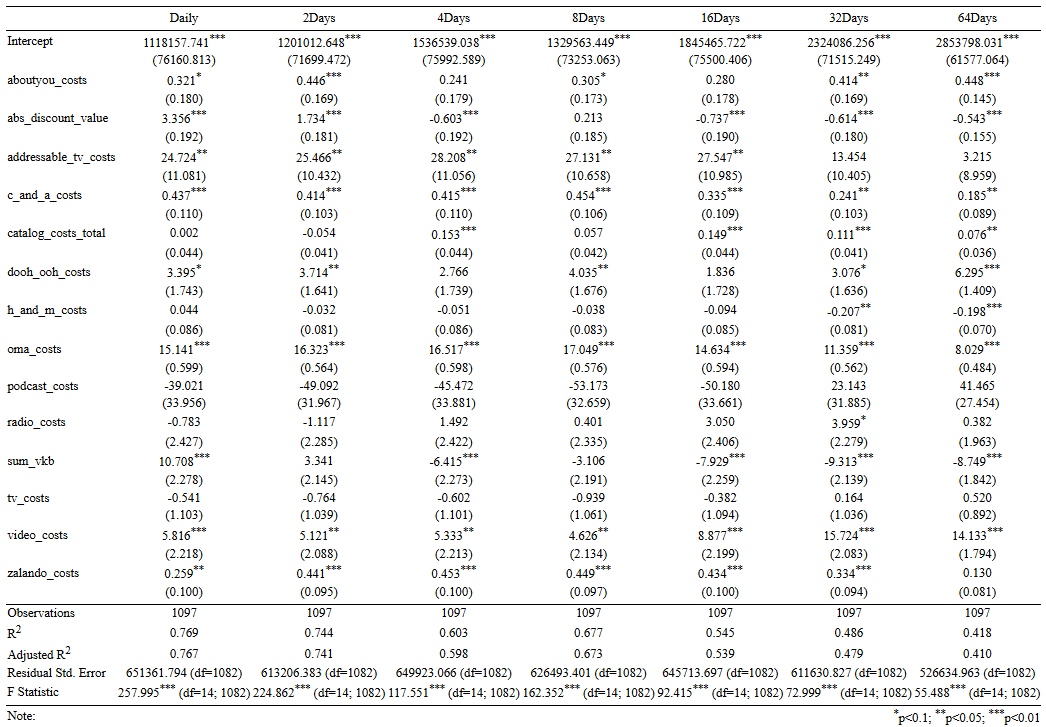
\includegraphics[width=1\linewidth]{images/ols2.png}
    \caption{\ac{OLS}-Modellergebnis ohne Saisonalität}
    \label{fig:OLSohneSaison}
\end{figure}
\noindent
Da \verb|pred_prophet| eine hohe Kollinearität erzeugt, wird diese Variable ausgeschlossen, und die Saisonalität wird auf alternative Weise in das Modell integriert. Der Nachfrageverlauf wurde deskriptiv analysiert und es wurde festgestellt, dass es wiederkehrende Muster gibt (s. \autoref{fig:saisonalitätlinien}). Beispielsweise bilden August und Januar die Tiefpunkte, während April bis Juni sowie September bis November die Hochpunkte der Nachfrage darstellen. Es wird vermutet, dass der Wechsel der Jahreszeiten diese Muster beeinflusst. Im Frühling, insbesondere in den Monaten April, Mai und Juni, gibt es eine Übergangszeit zwischen den kalten Wintermonaten und den warmen Sommermonaten. In dieser Zeit steigt die Nachfrage nach leichteren, dünneren Kleidungsstücken für die warmen Sommermonate. Umgekehrt steigt in den Herbstmonaten September, Oktober und November die Nachfrage nach wärmeren Kleidungsstücken wie Pullovern, Mänteln und Jacken als Vorbereitung auf kühlere Tage. Im Gegensatz dazu sind Januar und August Monate, in denen die Nachfrage nach Kleidung bereits gesättigt ist, da sie mitten in den kälteren bzw. heißeren Monaten liegen. Auch nach Erfahrung in der Abteilung gibt es am Wochenende eine erhöhte Nachfrage. \\\\
\begin{figure}[H]
    \centering
    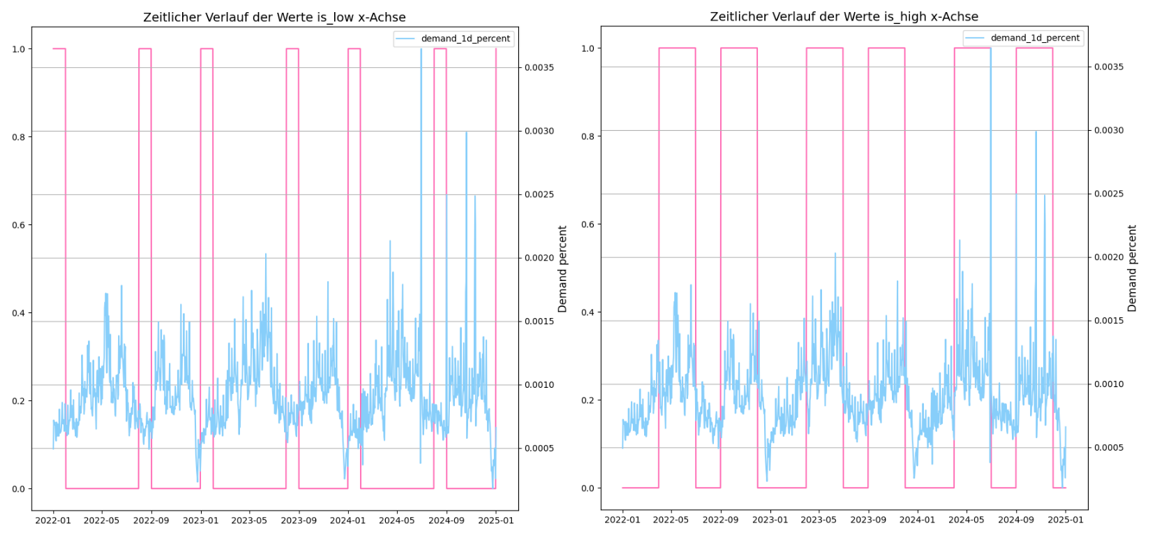
\includegraphics[width=1\linewidth]{images/nachfrageverlauf.png}
    \caption{Einführung der Saisonalität, eigene Darstellung}
    \label{fig:saisonalitätlinien}
\end{figure}
\noindent
Danach werden Variablen \verb|is_low|, \verb|is_weekend|, \verb|is_summer| und \verb|is_autumn| erstellt. Der Prädiktor \verb|is_low| kennzeichnet die Monate Januar und August, die Tiefpunkte in der Nachfrage aufweisen. \verb|is_weekend| beschreibt, ob das Datum auf ein Wochenende fällt. \verb|is_summer| und \verb|is_autumn| geben an, ob das Datum in einem der Sommer- oder Herbstmonate mit einem Hochpunkt der Nachfrage liegt. \verb|is_summer| umfasst die Monate April, Mai und Juni, während \verb|is_autumn| die Monate September, Oktober und November enthält. Diese Variablen werden in numerische Werte umgewandelt, wobei \verb|True| in 1 und \verb|False| in 0 umgewandelt wird. Ein Boxplot wird erstellt, um die Streuung der Nachfrage in Bezug auf diese Variablen zu visualisieren. In \autoref{fig:boxplotsaison} ist zu erkennen, dass das erste Quartil, der Median und das dritte Quartil der Nachfrage bei einem positiven Saisonalitätswert höher liegen. Das zeigt einen möglichen Zusammenhang zwischen der Nachfrage und den Saisonalitätswerten. Allerdings stellte sich in der deskriptiven Analyse heraus, dass \verb|is_low| eine hohe Kollinearität aufweist und daher ebenfalls entfernt wurde.
\begin{lstlisting}[language=Python, linewidth=\textwidth]
df_raw['is_low'] = df_raw['date'].dt.month.isin([1,8])
df_raw['is_weekend'] = df_raw['date'].dt.weekday >= 5  
df_raw['is_summer'] = df_raw['date'].dt.month.isin([4,5,6])  
df_raw['is_autumn'] = df_raw['date'].dt.month.isin([9,10,11]) 
\end{lstlisting}
\begin{figure}[H]
    \centering
    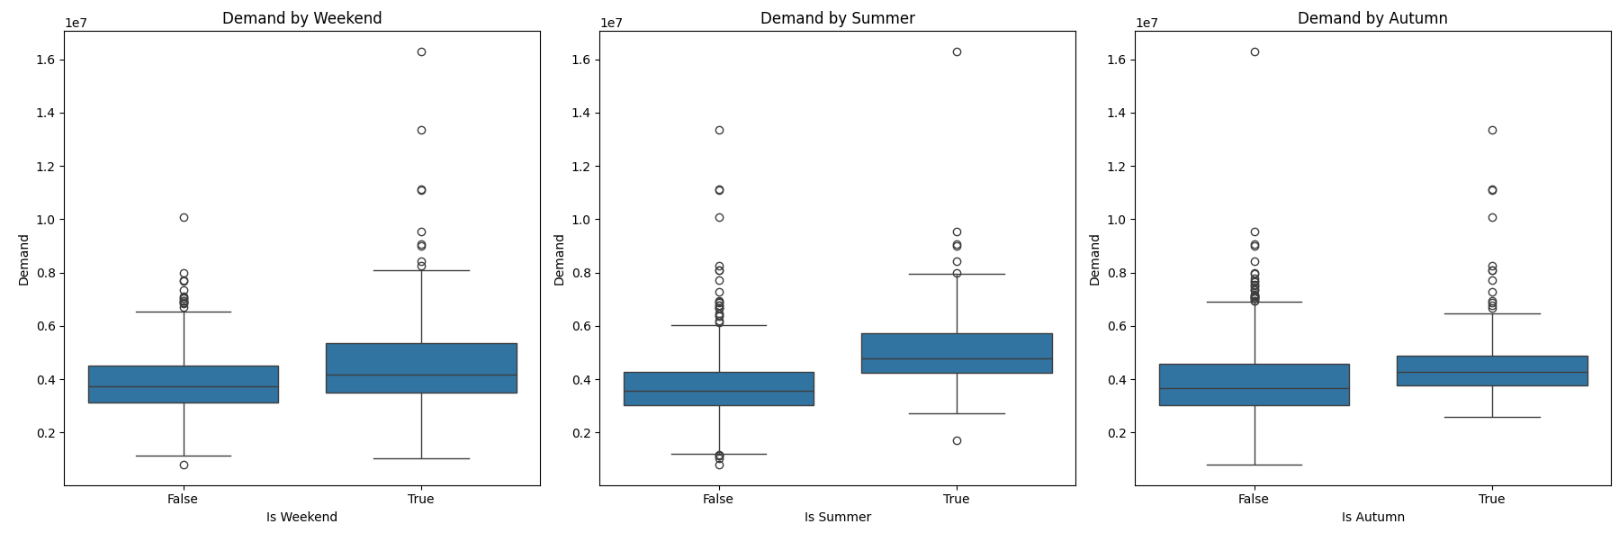
\includegraphics[width=1\linewidth]{images/boxplot.png}
    \caption{Boxplot: Nachfrage-Streuung mit Saisonalität, eigene Darstellung}
    \label{fig:boxplotsaison}
\end{figure}
In der weiteren Modellierung zeigen \verb|addressable_tv_costs| und \verb|podcast_costs| ebenfalls unrealistische Werte. \verb|addressable_tv_costs| weist einen \ac{ROAS} von -25 Euro auf, und \verb|podcast_costs| weist einen Wert von -101 Euro auf. Nach Rücksprache mit der Media-Abteilung stellte sich heraus, dass Podcasts nur aktiviert werden, wenn bonprix über zusätzliches Budget verfügt. Podcasts sind kostenintensiv und haben eine geringere Reichweite. Außerdem ist in \autoref{fig:mediapie} zu erkennen, dass \verb|podcast_costs| nur 0,7 \% der gesamten Mediaausgaben einnimmt und die letzte Aktivierung nach der deskriptiven Analyse im Mai 2022 stattfand. Daher wurde der Prädiktor \verb|podcast_costs| aus dem Modell entfernt. Das addressierbare TV sei eine kostengünstigere Variante des herkömmlichen TVs, und beide werden auf großen Bildschirmen genutzt. Da es für die Kunden ein ähnliches Erlebnis bietet, wurde empfohlen, sie zusammenzuführen. Nach der Fertigstellung der neuen Kombination der Prädiktoren wird das Modell erneut ausgeführt, und aus diesen finalen Ergebnissen wird im nächsten Kapitel eine Schlussfolgerung gezogen. 
\subsection{Schlussfolgerungen und Implikationen}
\label{schlussfolgerungenUndImplikationen}
Das finale Modell wurde mit den ausgewählten Prädiktoren aus dem letzten Kapitel erstellt. \\\\
In den Modellergebnissen wird festgestellt, dass die saisonalen Variablen \verb|is_autumn|, \verb|is_summer| und \verb|is_weekend| einen erheblichen sechstelligen Nachfrageeffekt aufweisen. 19 von 21 Werten sind mit drei Sternchen gekennzeichnet und somit hoch signifikant. Mit Ausnahme des Wertes von \verb|is_weekend| für die Zwei-Tage-Spanne, der keine Signifikanz aufweist. Es wird vermutet, dass dies darauf zurückzuführen ist, dass beide Werte ein Muster von zwei Tagen aufweisen. Das Bestimmtheitsmaß für längere Zeitspannen ist ebenfalls auf über 0,75 gestiegen, im Gegensatz zu dem früheren Wert von 0,418 ohne Berücksichtigung der Saisonalität.\\\\
Die Variablen \verb|oma_costs|, \verb|abs_discount_value| und \verb|sum_vkb| haben, wie erwartet, einen hohen Nachfrageeffekt auf Tagesebene. \verb|oma_costs| erklärt 12 Euro in der Nachfrage pro investiertem Euro, während \verb|sum_vkb| 14 Euro erklärt. \verb|abs_discount_value| hat ebenfalls einen signifikanten Effekt von 3,5 Euro. Allerdings nimmt der Nachfrageeffekt im Laufe der Zeit ab. \verb|sum_vkb| und \verb|abs_discount_costs| werden über eine Zeitspanne von 64 Tagen jeweils negativ, mit -3 Euro und -0,3 Euro. Es wird vermutet, dass Aktionen wie kostenloser Versand und Rabatte eine höhere, aber nicht nachhaltige Nachfrage erzeugen. Das bedeutet, dass Kunden in Zeiten niedriger Preise mehr kaufen und ihren Konsum für einen längeren Zeitraum einstellen. \\\\
Im Gegensatz zur Verkaufsförderung haben Media-Kanäle einen nachhaltigeren Verlauf. \verb|digital_video_display_costs|, \verb|dooh_ooh_costs|, \verb|tv_sum_costs| weisen anfangs einen niedrigeren Wert auf mit jeweils 2,68 Euro, 1,37 Euro und 0,5 Euro. In der Zeitspanne von vier Tagen senken \verb|digital_video_display_costs| und \verb|dooh_ooh_costs| jedoch auf jeweils -2,26 Euro und -1,86 Euro. In der letzten Zeitspanne von 64 Tagen steigen die drei Kanäle auf 6,8 Euro, 1,1 Euro und 2,15 Euro. Es wird vermutet, dass die Markenwerbung die Kaufentscheidung beeinflusst. Laut \autoref{MediaKanäleBeiBonprix} besteht das Ziel der Media-Kanäle in der Markenwerbung, wie der Steigerung der Markenbekanntheit und der Markenberücksichtigung.
\begin{figure}[H]
    \centering
    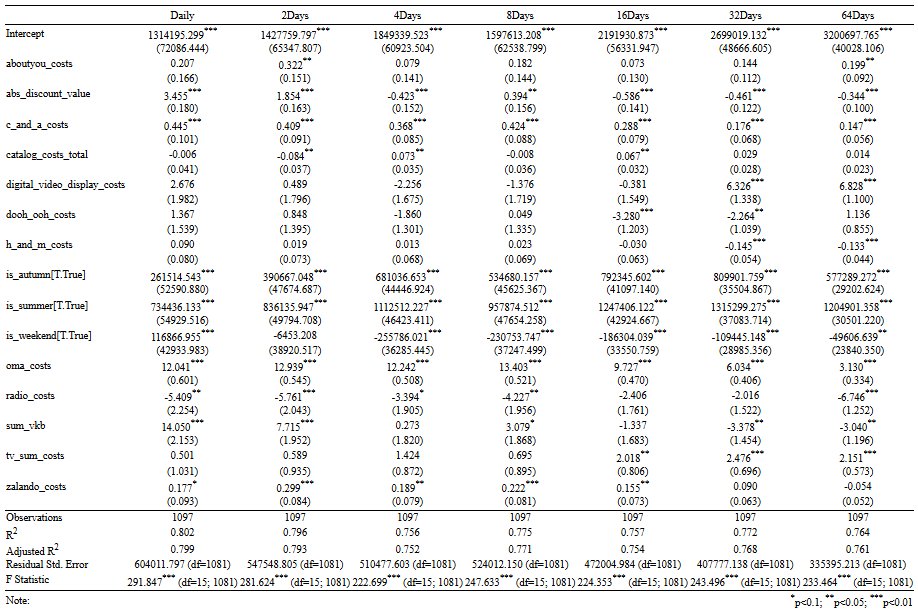
\includegraphics[width=1\linewidth]{images/finalols.png}
    \caption{Finales Modellergebnis mit \ac{OLS}}
    \label{fig:finalmodell}
\end{figure}

\begin{figure}
    \centering
    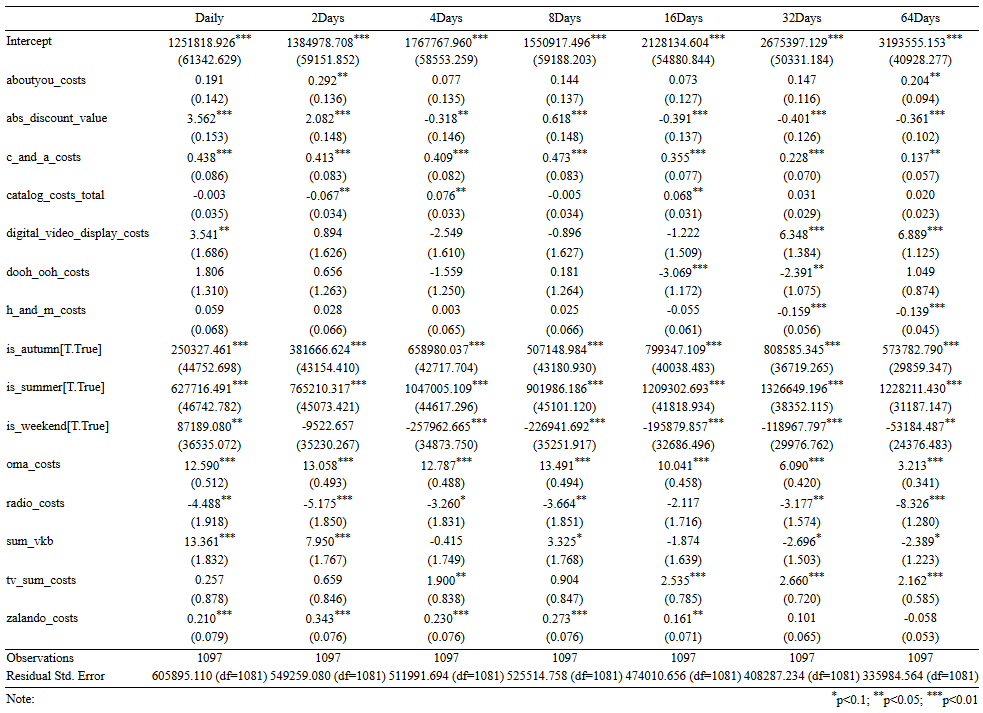
\includegraphics[width=1\linewidth]{images/finalhuber.png}
    \caption{Finales Modellergebnis mit der Huber-Loss-Funktion}
    \label{fig:finalhuber}
\end{figure}